\chapter{Benchmark Testing} \label{chap:benchmarks}
In this chapter a series of performance benchmarks are conducted. The benchmarks were intended to explore whether compilation technique has an effect on execution speed. In order to test this, the game engines Godot and CryEngine were used, as they both claim support for an interpreted (GDScript and Lua respectively), a \ac{JIT}-compiled (C\#) and a compiled (C++) language. Due to problems with both engines the focus switched and the chapter instead examines the performance of four different popular game engines; Unity, Unreal Engine, CryEngine and Godot.

We also wanted to explore if functional languages are slower than imperative languages. We do so to confirm or reject the popular belief we found that functional languages \dquote{suck} because they are slow \cite{pop:functional:sucks,pop:functional:slow} and hence cannot be used for game development. In this experiment we use the Arcadia plugin \cite{arcadia:github} for Unity and compare the execution speed of that with Mono C\# in Unity.

\section{Scripting vs. Engine}
In this section we explore whether the common hypothesis that \textit{\dquote{interpreted languages are slower than compiled languages}}\cite{IBM:Knowledgebase} is actually true. In this case we do so in the context of gameplay programming languages (as presented in \secref{gameplay:programming}). While common belief tells us that interpreted languages execute slower than compiled languages, there is little research to prove this claim. Furthermore the degree of difference in performance is interesting when considering the cost effectiveness of such systems.

\subsection{Platform}
In order to explore the claim a game engine that provides support for both an interpreted and a compiled language was needed. Two candidates that fulfil these requirements are Godot and CryEngine \cite{cryengine:home}.

On the features section of Godot Engine's website they promise:
\begin{itemize}
    \item GDScript Python-like scripting language [...]
    \item Full C\# 7.0 support using Mono.
    \item Full C++ support without needing to recompile the engine.
    \item ...
\end{itemize}
CryEngine promise support for C\#, C++ and ScriptBind (an \ac{API} for Lua) \cite{cryengine:languages}.

Both options sound very appealing for the test. As a first option Godot was chosen. The three languages supported (among many others) by Godot presents three different compilation strategies; GDScript is interpreted in the editor and \ac{JIT} compiled in release\cite{locurcio:gdscript}, C\# is \ac{JIT} compiled at runtime and C++ is compiled to machine code (which in Godot's case is called by another Godot scripting language: NativeScript). 

\subsection{Test setup}
We decided to use the \ttt{Mark8} benchmarking algorithm presented in \cite{sestoft2013microbenchmarks} (see also \secref{sestoft-scaffolding}). However, as GDScript does not currently have a native stopwatch implementation, a custom stopwatch was implemented. This stopwatch contains the following methods:
\begin{labeling}{\quad\quad}
    \item[Start] Starts the stopwatch by reading the current system time in the finest possible granularity since the game started and storing it in a variable, \ttt{start\_time}.
    \item[ElapsedTime] Calculates the elapsed time by subtracting \ttt{start\_time} from the current time and thereafter converting to nanoseconds.
\end{labeling}
In order to establish a common foundation for the tests a similar stopwatch-class was also implemented in C\# and C++. The only difference between the implementations are that C\# and C++ natively support counting in nanoseconds, whereas GDScript counts in miliseconds. There is, of course, a loss of precision in the GDScript implementation but it must suffice. 

Another thing that proved troublesome was that GDScript does not have first-class functions. This is required by Sestoft's algorithm, such that the timing code can be reused over multiple different tests. GDScript does, however, provide a way of packing a function into an object using \ttt{FuncRef} \cite{godot:funcref}. The packing takes as argument an object reference and the name of the function and does as such not have a direct reference to the function. How much overhead there is in looking up and invoking such function compared to C++'s and C\#'s high-order functions is unknown and might affect the running times.

Apart from said two problems, the \ttt{Mark8} algorithm could be directly translated to the three target languages.

\subsection{Method}
According to the findings in \cite{vmwarmup} a virtual machine have a startup time, wherein it doesn't reach peak performance. We expect the same to be the case for engine startup time. In order to avoid running the tests while the engine and virtual machine is starting up, a small test-runner was written. The test-runner starts the tests when the Space button is clicked. When the tests were run, we started the engine and waited three to five seconds before pressing space and starting the tests.

To the extent it was possible, the test-runner would output \ac{CSV}-files containing the data for each language. Another small script to merge and format the data was also written, which made it easier to work with the data.

\subsection{False Promises}
The implementation of the test cases was simple in GDScript, however, as the implementation proceeded to C\# and C++ problems started to occur. First and foremost, the \textit{\dquote{full C++/C\# support}} promised by Godot was not so full in the end. As of the time of writing, the C\# support is only a partial implementation of the Mono runtime, which in and of itself is a partial implementation.

As for C++, Godot uses another scripting language called NativeScript, which can dynamically load compiled code from C, C++, D, Nim and basically any language that can link to a C \ac{ABI}. However, NativeScript is in a very early stage and is undergoing frequent changes. While there exists a large corpus of guides and tutorials, they where contradictory and/or outdated.

We did not succeed in finding a solution and was left with the option of benchmarking GDScript against a partial C\# implementation. We agreed that this benchmarking would not provide any useful information and decided to switch to a different approach.

\subsection{CryEngine}
As a second approach CryEngine was examined. This involved porting the code to Lua and creating game projects for the C++ and C\# code. Luckily, the C++ and C\# code could be reused from the previous experiment with very little modification. However, as we proceeded with the Lua implementation it turned out that Lua had been deprecated in CryEngine V5.3 in favour of C\# and Lua support had been (seemingly) completely removed in V5.4 \cite{perkins:cryengine}. This rendered us unable to benchmark an interpreted language in the context of CryEngine.

\subsection{Summary}
As none of the two game engines that where selected for this experiment turned out to provide a useful framework for this test, we decided to take a different approach, which is presented in the following section. Furthermore, it would seem that interpreted languages are loosing favour and are been replaced by \ac{JIT}-compiled languages in many engines. In the engines presented in this report, Unity has deprecated JavaScript and Boo in favour of C\# \cite{fine:unityscript, unity:boo} and CryEngine has replaced Lua in favour of C\#\cite{perkins:cryengine}.
\section{Test Setup}
In this section we discuss the foundation for the microbenchmarks. We discuss first an important consideration to take when comparing languages, warmup time for \ac{JIT}-compiled and interpreted languages and thereby classify the different types of benchmarks that exist. Afterwards we discuss the platforms that are put to test and the system on which the tests were executed.

\subsection{Virtual Machine Warmup}\label{sec:sub:vmwarmup}
When making benchmarks it is important to take into account different factors that might affect the test's speed.
The example in this section will be the \textit{warmup} of virtual machines \cite{vmwarmup}.
The virtual machines that use \ac{JIT} compilation might recompile parts of the program that is run repeatedly, resulting in a speedup.
In \cite{vmwarmup} the authors test the hypothesis: \dquote{Small, deterministic programs reach a steady state of peak performance.}
To test this hypothesis they constructed some software to aid them in benchmarking called \textit{Krun}.
Krun manages the machine while the benchmarks are running, doing things such as: stopping userland daemons and network cards, rebooting the machine before every process execution and ensuring a consistent temperature before execution.

\btc{Hvad betyder disse tal? Hvem er 'They'?}They found out that only 43.5\%, 43.4\% and 30\% respectively, for three different systems actually provide \squote{good} warmup. The rest of processes either slowdown, never reach a steady state of performance or some mix of those two.

This means that counting on \acs{VM}s to speed up during execution is risky.
The startup time of \acs{VM}s should also be taken into consideration, as the startup time may reach as high as several seconds for some \acs{VM}s.

In order to alleviate this uncertainty with \acs{JIT}s we use macrobenchmarks. The bigger tests should provide a more realistic use case and therefore more realistic data.\btc{Dette afsnit bør komme efter 'Types of Benchmark'}

\subsection{Types of Benchmark}
In this report we concern ourselves with three types of benchmarks; micro-, macro- and application-benchmarks. This section provides the definitions of these benchmarks. In general benchmarks are tests run on computer programs, that yield some metric. This metric can be memory usage, run time or throughput \cite{Fleming:1986:LSC:5666.5673}. In this report we divide benchmarks into three categories that are distinguished by the size of the program under test.

\begin{description}
    \item[Micro] benchmarking, also known as component benchmarking, has been partially covered in \secref{micro-benchmarking}, however \secref{micro-benchmarking} focuses on how to microbenchmark rather then what microbenchmarking is. We have defined microbenchmarks as \textit{a benchmark testing a single and minimal unit of functionality and excluding start-up time}. In this case unit of functionality is a single function, object, or equivalent programming construct, of small size. The goal is to test the performance of the single unit.
    \item[Macro] is defined as \textit{a benchmark testing multiple units of functionality and excluding start-up time}. The main difference between micro and macro benchmarking is the number of functional units. The goal of macro benchmarking is to test the performance of a set of connected units.
    \item[Application] benchmarking, also known as real program benchmarking, is the largest category of benchmarks. They are defined as \textit{a benchmark testing a full application, consisting of multiple units of functionality and including start-up time}
\end{description}

\subsection{Platforms}
This experiment examines C++, C\# and Clojure along with four popular game engines that support the chosen languages. As a baseline comparison, the same tests are run natively on the machine. For C++, CryEngine and Unreal Engine were the engines of choice. For C\#, we chose Unity and Godot and CryEngine. For Clojure, we used a Unity plugin called Arcadia \cite{arcadia:github}, which gives access an interpreted version of Clojure in Unity. For the native baseline, both the Mono and .NET Core runtime where tested for C\#. For C++, Microsoft's Visual C++ compiler was tested as it is supported in Windows. \ac{GCC} cannot be ignored when talking about C++, but the problem is that it requires a Unix-like system. There are a couple of choices here; MinGW, CygWin or \ac{WSL}. As \ac{WSL} is the most convenient platform to setup, we chose that one (the choice of \ac{WSL} is discussed in \secref{micro:threats}). Furthermore, the list of platforms and engines can be seen in \tableref{sut}

\makeTable{
{| l | c | c |}
\hline
\textbf{Engine} & Debug/Editor & Release \\ \hline
Dotnet & \checkmark & \checkmark \\ \hline
Mono & \checkmark & \checkmark \\ \hline
Unity & \checkmark & \checkmark \\ \hline
Godot & \checkmark & \checkmark \\ \hline
GCC C++ (\ac{WSL}) & \checkmark & \checkmark \\ \hline
Visual C++ & \checkmark & \checkmark \\ \hline
Unreal & \checkmark & \texttimes \\ \hline
CryEngine (C++) & \checkmark & \checkmark \\ \hline
CryEngine (C\#) & \checkmark & \texttimes \\\hline
Arcadia (Clojure) & \checkmark & \texttimes \\\hline
}{Systems under Test}{sut}
In the ideal case all boxes in \tableref{sut} would be ticked, but due to complications with the build process, we were unable to test Unreal in release mode along with CryEngine (C\#) in release mode. As for Arcadia, it is in an early stage of development, and we were thus unable to build a functioning release build.

\subsubsection{System Setup}
The system on which the tests were executed runs Windows 10 Pro and its specifications are listed in \tableref{sys-specs}.

\makeTable{
{| l | R{6em} | p{3em} |}
\hline
\multicolumn{3}{| c |}{\textbf{Processor}} \\ \hline
Model & \multicolumn{2}{| l |}{Intel Core i7 4702HQ} \\ \hline
Clock Frequency & 2.2 & GHz \\ \hline
Max Turbo & 3.2 & GHz \\ \hline
Physical & 4 & Cores \\ \hline
Logical\footnotemark & 8 & Cores \\ \hline
\multicolumn{3}{|c|}{\textbf{Memory}} \\ \hline
Memory Size & 16 & GiB  \\ \hline
Memory Speed & 1600 & MHz \\ \hline
Memory Type &  \multicolumn{2}{| l |}{DDR3L 1600} \\ \hline
}{System Specifications}{sys-specs}\footnotetext{Logical cores are sometimes called threads. However logical cores is used here to avoid confusion with the software concept; threads, which is distinct from hardware threads.}

\subsubsection{Functional Clojure} \todo{This section comes out of nowhere. It needs a better lead-in or should be moved somewhere else.}
The Clojure language is a LISP-style functional language that runs on the \ac{JVM} \cite{clojure:about}. Arcadia uses a version of Clojure that is ported to the .NET virtual machine and is thus compatible with Unity and is interpreted. This allows the use of functional programming in Unity. However, some of the microbenchmarks that were chosen here are hard to implement with a pure approach. First and foremost, several of the tests require the use of mutable variables. In order to satisfy this we use the state management system provided by Arcadia. This allows the use of mutable variables stored as a state for a specific object in Unity. 
We suspect that using this introduces a large overhead, but were unable to find sources that says so.
We also make use of the \texttt{do} keyword in Clojure, which allows sequential execution of functions, further distancing this test from a functional approach.

Arcadia is integrated with Unity in a way that allows the use of Unity's .NET libraries in Clojure.
These are used in several places, but we are not certain if there is a performance overhead by using them.
Their usage, again promote using Clojure in a non-functional manner. 

With these arguments in mind, we make no claim to use Clojure 'correctly' or in a truly functional way.

\subsection{Classifications}
In this section we will classify the languages of the different game engines according to the classification presented in \cite{5962102}, which was summarised in \secref{gameplay:programming}. We do not classify the languages that are in beta at the time of writing. The classifications are displayed in \tableref{benchmark:classification}.

The classification system presented in \cite{5962102} classify the properties of the languages used in the scripting system. As we have seen previously in the report, many scripting systems have been replaced with C\#, meaning that all scripting systems presented here would be classified as regular scripts. We therefore adapt the definition to instead examine the properties of the game engines' scripting system (i.e. the classes declared by the game engine, the game engine's \ac{API} and intended use of the scripting language). 

\makeTable{
{| l | l | l | P{.4\textwidth} |}
\hline
\textbf{Engine} & \textbf{Language} & \textbf{Classification} & \textbf{Reasoning} \\\hline
Unity           & C\#       & Regular Script & Coroutines can run code outside \unity's update events. \\ \hline
Unreal Engine   & C++       & Event Oriented & Custom events, but all code runs with Unreal Engine's \ttt{Tick}. \\ \hline
Unreal Engine   & Blueprint & Event Oriented & Custom events, but all code runs with Unreal Engine's \ttt{Tick}\\ \hline
CryEngine       & C\#       & Event Oriented & Custom events, but all code run with CryEngine's \ttt{OnUpdate}. \\ \hline
CryEngine       & C++       & Event Handler & No language support for events, but all code runs with CryEngine's \ttt{ProcessEvent}. \\ \hline
Godot           & C\#       & Event Oriented & Godot uses signals to parse messages between components, but all signals are sent from Godot's \ttt{\_Process}. \\ \hline
Godot           & GdScript  & Regular Script & Same as for C\#, but GDScript supports threads that can run functions asyncronously from the game loop. \\ \hline
Godot           & NativeScript & Initialisation & NativeScript may only be used to import compiled code written in e.g. C or C++. \\ \hline
}{Scripting system classifications, categories taken from \cite{5962102}}{benchmark:classification}


An example of a game engines' \ac{API} towards the language is \unity's \ttt{MonoBehaviour}s. \ttt{MonoBehaviour}s in \unityspace may declare a set of methods that are invoked while the game is running \cite{unity:monobehaviour}. Examples of these are \ttt{Start}, \ttt{Update} and \ttt{OnDestroy} that are called when respectively when the game starts, each time a frame is generated and when the MonoBehaviour is removed from the game. Unity also supports events declared in scripts \cite{unity:event}. Other scripts may subscribe to these events to be notified when they occur. These, unlike the classification in \cite{5962102}, are not imported into the game engine when the game starts, but are rather handled from the scripting system.

The reason \unityspace ended in the regular script category is because of \ttt{Coroutines} \cite{unity:coroutines}. \ttt{Coroutines} are used to carry out tasks that happen over a period of time or periodically without cluttering the \ttt{Update}-method. By default, a coroutine is called once every frame, but there exists constructs that allow the programmer to specify that the coroutine be called more rarely (e.g. every fifth frame or every 0.5 seconds). We do not classify this as regular scripts, because of their tight connection with the game loop and the fact that they are not stand-alone scripts.
\section{Micro-Benchmarks}
In this experiment we examine four different game engines; Unreal Engine, Unity, CryEngine and Godot. The following research questions formulate the foundation of the experiment:
\begin{itemize}
    \item Are compiled languages (in this case C++) in fact faster than their interpreted and \ac{JIT}-compiled counterparts?
    \item Does a game engine's runtime have a negative effect on a game engines performance in comparison to its native performance\footnote{By native we mean the language in it's default runtime}?
    \item In the context of Unity, does the use of a functional language (Clojure) increase execution time?
\end{itemize}

\subsection{Test cases}
The test cases were created to explore some different aspects of a gameplay programming language. The test cases are as follows: 
\begin{description} 
    \item[Sestoft's multiply] Sestoft's \ttt{multiply}-method is listed in \lstref{sestoft:multiply}. This method is designed to prevent compilers from optimising the multiplication away with a constant value as well as keeping the input relatively small.
    %\item Sum all elements of a matrix
    \item[Vector math] In this microbenchmark, a series of vector operations was tested; i.e. Scaling a vector by a factor, Multiplying two vectors, translating a vector, subtracting two vectors, calculating the length of a vector, calculating dot product of two vectors.
    \item[Array Allocation] In Array Allocation an array of 100,000 elements should be allocated and initialised to 0 and the last element returned.
    \item[Primes100] In Primes100 the Sieve of Eratosthenes algorithm\cite{eratosthenes:sieve} should be implemented and generate all prime numbers that are lower than 100. This produces a list of numbers, the last of which are returned from the function. 
    %\item Side-scroller player control code
\end{description}

\begin{lstlisting}[label={lst:sestoft:multiply}, caption={Sestoft's proposed benchmarking method}, language={Java}, style=java-highlight]
private static double multiply(int i) {
    double x = 1.1 * (double)(i & 0xFF);
    return x * x * x * x * x * x * x * x * x * x * x * x * x * x * x * x * x * x * x * x;
}
\end{lstlisting}

For the vector calculations, the engines' implementation were used. In order to support the native platforms we chose two vector libraries; \ttt{Boost} for C++ \cite{cpp:vector} and \ttt{System.Numerics} for C\# \cite{system:numerics:vectors}. The reason for choosing Boost for C++ is that it is widely used, for instance in Unreal Engine's own vector implementation. Another viable option was to use Lumberyard's vector implementation \cite{lumberyard:vector}, which is also open source. For C\# we chose to use \ttt{System.Numerics.Vector<T>} because it is included in the standard library. The \ttt{System.Numerics.Vector<T>} is implemented to use \ac{SIMD} calls to improve performance \cite{msdn:vectors}.

\subsection{Results}
In this section the results of the test cases are shown and discussed. The most prominent results have been selected and listed in \tableref{benchmark:release-results}, \figureref{scale2d-res} and \figureref{mem-test-res}. The results from all tests may be found in \appendixref{benchmark-res}. All tests results are listed as mean running time in nanoseconds and the graphs use logarithmic scale on the y-axis, as the running times vary wildly between the platforms. 

\textbf{\begin{table}[H]
    \sisetup{round-mode=places}
    \rowcolors{1}{}{lightgray}
    \makebox[\textwidth][c]{
    \begin{tabular}{| P{2.2cm} | S[round-precision=2] | S[round-precision=2] | S[round-precision=2] | S[round-precision=2] | S[round-precision=2] | S[round-precision=2] |}
        \hline
        \textbf{Test case} & \textbf{Dotnet} & \textbf{Mono} & \textbf{Unity} & \textbf{C++}
        \csvreader[head to column names]{benchmark-tab.csv}
        {1=\cases, 5=\dotnet, 7=\mono, 3=\unity, 13=\godot, 12=\cpp} % <Column number>=<Macro>
        {\\\hline \cases & \dotnet & \mono & \unity & \cpp}
        \\ \hline
    \end{tabular}}
    \caption{Release Benchmark Results, results listed in runtime in nanoseconds}
    \label{tab:benchmark:release-results}
\end{table}}

\figureref{scale3d-res} was selected as an example of how the running times are distributed over the platforms. The first thing to notice is that in most cases the running time decreases drastically from running in debug/editor-mode versus running in release-mode. This was, however, not the case for Mono, Godot and to some extent Unity. Taking into account that both Godot and Unity runs on the mono platform, it is not strange that their performance reflect that of Mono. It seems, comparing Mono with Dotnet, that Mono fails to optimise the code as much for release builds.

\figureref{mem-test-res} shows the results from Array Allocation. The next thing to notice is that native C++, in all cases but Array Allocation, runs slower that both Dotnet and Mono.  But that can be attributed to the fact that it was run under \ac{WSL}. This is especially true, as Unreal Engine ranks as the most performant of all competitors in the debug-category.
%Unreal Engine does not compete in the release-category, as we did not succeed in neither running, nor outputting running times after building the project in release-mode.

\benchmarkRes{Scale Vector 3D}{scale3d-res}

Among the game engines Unreal Engine ranks the highest - it even ranks higher in debug-mode than all the other engines do in release-mode. This could indicate that either there is some truth to the common belief that C++ is the fastest language for game development or that Unreal Engine's C++ implementation is far better optimised than any other platform in this experiment. 
One thing to notice, however, is that Unreal Engine fails to optimise the Array Allocation, which was the case for both Visual C++ and \ac{GCC} C++.

\benchmarkRes{Array Allocation}{mem-test-res}

The performance benchmarks was only run once for each platform, but the design of the benchmark takes this into account by running each test multiple times.

\subsection{Threats to Validity} \label{sec:micro:threats}
In this section the methods used to obtain the results and the results themselves are examined to uncover potential threats to validity. We will examine the internal and external validity of the results; where the internal validity can summarised as whether the tests measure what it is intended to measure. The external validity is whether the utilised test cases apply to other cases in the field.

\subsubsection{Internal Validity}
The major threats to the internal validity is that many compilers perform some optimisation of code regardless of optimisation settings. An example of this is the C function in \lstref{bad-c}. The compiler will instead replace all calls to this function with the literal four. This removes a function call and is desirable for programs in general, but not benchmarks. It is vital that the benchmark does not take shortcuts when running, otherwise results are skewed.

\begin{lstlisting}[language=C,label={lst:bad-c},caption={An example of Function Inlining}]
int bad_func(){
    return 4;
}
\end{lstlisting}

In order to deal with the internal threats we have examined our results and looked for unexpected results. Such results are examined in detail to verify that they are genuine or a faulty measurement. During the initial implementation of the tests these themes where kept in mind. Finally, we have examined the following issues.

\begin{description}
    \item[\textbf{Array Allocation}]
    C\# is a managed language which means that it is impossible to allocate an array without also initialising each element in the array. In C++ it is possible to allocate an array without initialising each element and also possible to initialise each element. To make the compared functions more similar, we chose to initialise the array in both C\# and C++. It can be argued that in C++, it will not always make sense to initialise each element, but as there also are many cases where initialising each element would be most sensible. Another test could be added to compare C++ with uninitialised arrays against C\# to examine the effect of that.
    \item[\textbf{Windows Subsystem for Linux}]
    All the benchmarks are run on the same computer and in the same \ac{OS}, however, as \ac{GCC} is not implemented on Windows, \ac{WSL} was used. Initially we where worried that this would incur a significant overhead that might skew results, however, research showed that \ac{WSL} performs almost as well as bare metal Linux distributions \cite{phoronix:wslperformance}. The only significant difference was \ac{I/O} which is not used during the micro-benchmarks themselves.
    \item[\textbf{Skill Level}]
    The tests were implemented by the authors of this report, who have different experience levels with the languages. All authors have experience with C\#, but few have C++ experience. This has effected test implementation time and may have effected the efficacy of the tests themselves. To mitigate this, we have used online resources and followed best practice.
\end{description}

\subsubsection{External Validity}
The primary external threat is whether the selected test cases are properly selected. If the tests are improperly selected they may not be representative of actual game engine workloads or maybe the test cases are local maxima or minima. Internal threats can in this case be examined and determined to be correct or incorrect, however, this is not the case for the external threats. It is very difficult to prove the non-existence of local maxima and minima\btc{??}.\todo{Discuss validity of test selection}


\section{Macrobenchmarks}\label{sec:macrobenchmarks}
In order to not skew results towards \ac{JIT} compilers, because microbenchmarks are likely to be misleading \cite{sestoft2013microbenchmarks, microbenchmarkmislead}, we also implemented a macrobenchmark.
Some sources claim that \ac{JIT} provides speedup on loops, although according to a recent study this is not always the case \cite{vmwarmup}.

\subsection{Test Cases}
We defined a macrobenchmark as \dquote{\textit{a benchmark testing multiple units of functionality and excluding start-up time}}. As we have not been able to find any specific definition of macrobenchmarks in scientific literature, we decided to brainstorm some ideas. The ideas are as follows:
\begin{description}
    \item[Angry Physics] This test case is reminiscent of the game Angry Birds, hence the name. In this test a series of 3D objects (boxes, balls, pyramids, etc.) is placed on a platform. A canon that shoots is place at a distance from the platform. This canon will shoot projectiles of different size, mass and shape at the platform to trigger collisions and gravity simulation.
    \item[Wumpus World] In this case a 2D grid-based board is placed in the world. In the world an agent must collect a treasure and return to the start. The world is also inhabited by wumpuses, that wish to eat the agent. There are also a series of pits which the agent must avoid. The agent can sense wumpuses and pits on neighbouring grids by stenches and breezes respectively \cite{wumpus:world}.
    \item[Cowichan Problems] The Cowichan problems is a series of thirteen problems that mainly revolves around matrix and vector calculations \cite{wilson1995assessing}. The sizes of the matrices and vectors can be scaled to fit the size of the test and the problems chained to test different aspects of a language.
    \item[Game of Life] Game of Life is a cellular automaton described by John Conway \cite{game:of:life}. In the game organisms can be placed in a grid world. There are a series of rules, that determines how the organisms will evolve or die, that needs to be evaluated for each organism.
\end{description}

% Wumpus world: http://aima.cs.berkeley.edu/slides-pdf/chapter07-6pp.pdf
% Lund Universitet Applied Artificial Intelligence: http://cs.lth.se/edaf70/course-material/
We chose to implement the Wumpus World, as this macrobenchmark involves a set of classes including e.g. wumpus, world and agent. Furthermore, it is somewhat reminiscent of a game, being that it has an \ac{AI}-element along with the possibility of adding graphics. Even though it is a simulation of an \ac{AI} it has a deterministic behaviour on a given map.

\subsection{Rules in Wumpus World}
The Wumpus World is an N x M grid world. Each cell may contain one object. The Wumpus World uses the term \textit{neighbouring cells}. Given a cell X, it's neighbouring cells are that to the north, east, south or west of X. The cells on the diagonal are not considered neighbours. A visual representation, as presented in \cite{wumpus:world}, is shown in \figureref{wumpus:world}. A Wumpus can give off a stench so the agent know where the Wumpus could be, the same goes for for pits that have breezes next to it. Last there is Glitter which is the treasure, the agent wins when it gets back to start position (0,0), with the treasure.

\begin{figure}
    \centering
    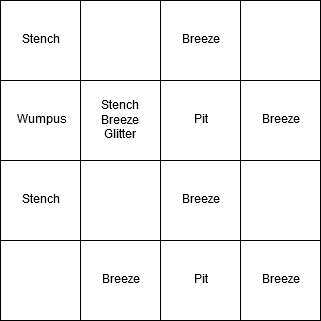
\includegraphics[width=.5\textwidth]{images/wumpus.png}
    \caption{A 4 x 4 Wumpus World with one Wumpus and two pits \cite{wumpus:world}}
    \label{fig:wumpus:world}
\end{figure}

An agent may take one of a couple of actions in each turn. They are as follows:
\begin{description}
    \item[Forward] The agent moves one step forward in its current direction.
    \item[Turn] The agent turns either left or right to change its direction.
    \item[Grab] The agent picks up the content of the current cell.
    \item[Release] The agent releases what ever it is holding and places it on the current grid cell.
    \item[Shoot] The agent shoots an arrow forwards from its current position to kill a wumpus in front of it.
    \item[Climb] The agent may climb out of the cave if it's located in the start position.
\end{description}

The agent is \dquote{blind} and may only perceive the world through percepts. The percepts are tied to objects, which are as follows:
\begin{description}
    \item[Agent] The agent is an \ac{AI}. It has a starting position and a goal of retrieving a treasure in the world. It must do so while minimising the score, i.e. the number of actions it has taken.
    \item[Wumpus] Wumpuses are hostile towards the agent. If the agent ends up in the same cell as a Wumpus, it will die. Wumpuses give of stench to the neighbouring cells. If the agent is sure of the location of a Wumpus, it may shoot to kill it (in which case the agent perceives a scream).
    \item[Pit] A pit is a hole in the ground. The agent will die if it falls into a pit and pits give of a breeze to neighbouring cells.
    \item[Treasure] There is one treasure in each map. The agent has the goal of getting to the treasure, picking it up and going back to the start state. A treasure gives off glitter to the cell it is placed in.
\end{description}
Apart from said percepts, the agent will perceive a bump if it walks into a wall.

\subsubsection{Simplifications}
In the implementation we make a couple of simplifications from the description in \cite{wumpus:world}. The first is that we abstract away the bump perception and instead assume that the agent knows its current position in the world.
The agent also knows where it has been, so it remembers its path.

Regarding the agent's actions several changes were made. We did so because the actions presented in \cite{wumpus:world} seemed a bit terse, most likely because they are meant to represent an actual robot. As a precise robot simulation is not desired in this case, we argue that the simplifications won't do any harm\todo{Meh. We should probably write something more scientific here.}. The actions were changed as follows:
\begin{description}
    \item[Grab and Release] The grab and release actions are replaced with a Boolean flag to indicate whether or not the agent has reached the cell that holds the gold. If the agent is in the start cell with the flag set to true, the map is completed.
    \item[Turn and Forward] The turn and forward actions are replace with a \ttt{Move(direction)}-action, that moves the agent in the given direction. Direction either being north, west, east or south.
    \item[Climb] Finally the Climb action was removed and instead a map is completed when the agent reaches back to the start cell or dies from walking into a pit or a wumpus.
\end{description}

\subsection{Platforms}
We chose Unity and Unreal for the test. Unity was chosen because it, according to statista.com in 2014, was used by 62\% of the responses in their survey \cite{gameengine:statista}.
Unreal was chosen because it was the fastest of all the engines in the microbenchmarks (see \secref{micro-benchmarking}).

\tmc{Write an explanation as to why we do not include a functional language}
%In this experiment we do not include a functional language, as we were not able to find a game engine with a functional language and Arcadia's res.

\subsection{Metrics}
Unlike the microbenchmarks that had a predefined metric of measuring time, macrobenchmarks does not. In order to formulate a baseline for the discussion on which metric to use, a series of questions were formulated:
\begin{itemize}
    \item How many worlds can we spawn at once while still producing at least 60 \ac{FPS}?
    \item How many turns can we execute per second?
    \item How much time does one tick take?
    \item What is the memory footprint per Wumpus World?
\end{itemize}
The first question is tied to the fact, that the macrobenchmark is run in a game engine. In the context of games it makes sense, as it is the metrics most often used by gamers. However, it make less sense if the macrobenchmark is not intended to test a game engine.

The second question is also directly related the behaviour of game engines, but is disconnected somewhat from the user experience. Instead this is a measure of the raw computational throughput. \todo{This is thin.}

The third question has the advantage, that it pairs well with the metrics used in the microbenchmarks and the fourth, that memory is also a performance concern, that we have only briefly discussed previously in this project.

We choose to examine the last two questions by reusing the timer code that was written for the microbenchmarks along with examining memory use per instance of the wumpus world. The timing code was use to measure how long time each invocation of the \ttt{World}'s \ttt{Iterate}-method took. The \ttt{Iterate}-method is responsible for all Wumpus World-related logic, such as generating percepts for the agent, updating the agent's perceived world state etc. The test would run until the agent found the treasure and made it back to its start position. This was repeated 10 times for the same map. 

In performance benchmarking memory is naturally also of great concern, however, we could not find a meaningful way of measuring memory usage in Unreal Engine at the time of writing. Unreal Engine has a profiler tool that can measure the time it takes to generate a frame, but it's memory section is currently work-in-progress \cite{unreal:profiler}. The current state of the profiler plots a graph with frame count along the Y-axis and time along the X-axis. It provides an overview of all memory consumption in the game, but when they are plotted on the graph, they are so using frame count and time. Furthermore, it was not possible to plot one single graph over all memory consumption, but only for each component (of which there are around 200 in the profiler tool). Left with the option of examining Unity's memory without possibilities for comparison, we decided that memory benchmarking be left as future work.

\subsection{Results}
The results from the macrobenchmark is plotted in \figureref{macro-results}. The spikes in Unreal Engine's performance (iteration 14, 28 etc.) correspond to clearing the agent's state and beginning the next iteration. In the case of Unity, the execution time for the agent's first tour through the map is much higher than that of Unreal Engine. The execution time in Unity stabilises in the third iteration, approaching Unreal Engine's performance. Interestingly, the spikes that correspond to starting over are higher in Unreal Engine than they are in Unity. This comes at the cost of Unity's execution time spiking when not clearing the map, which could be caused by garbage collection. Generally Unreal Engine's execution times are more stable and predictable than those of Unity.

\begin{figure}
    \centering
    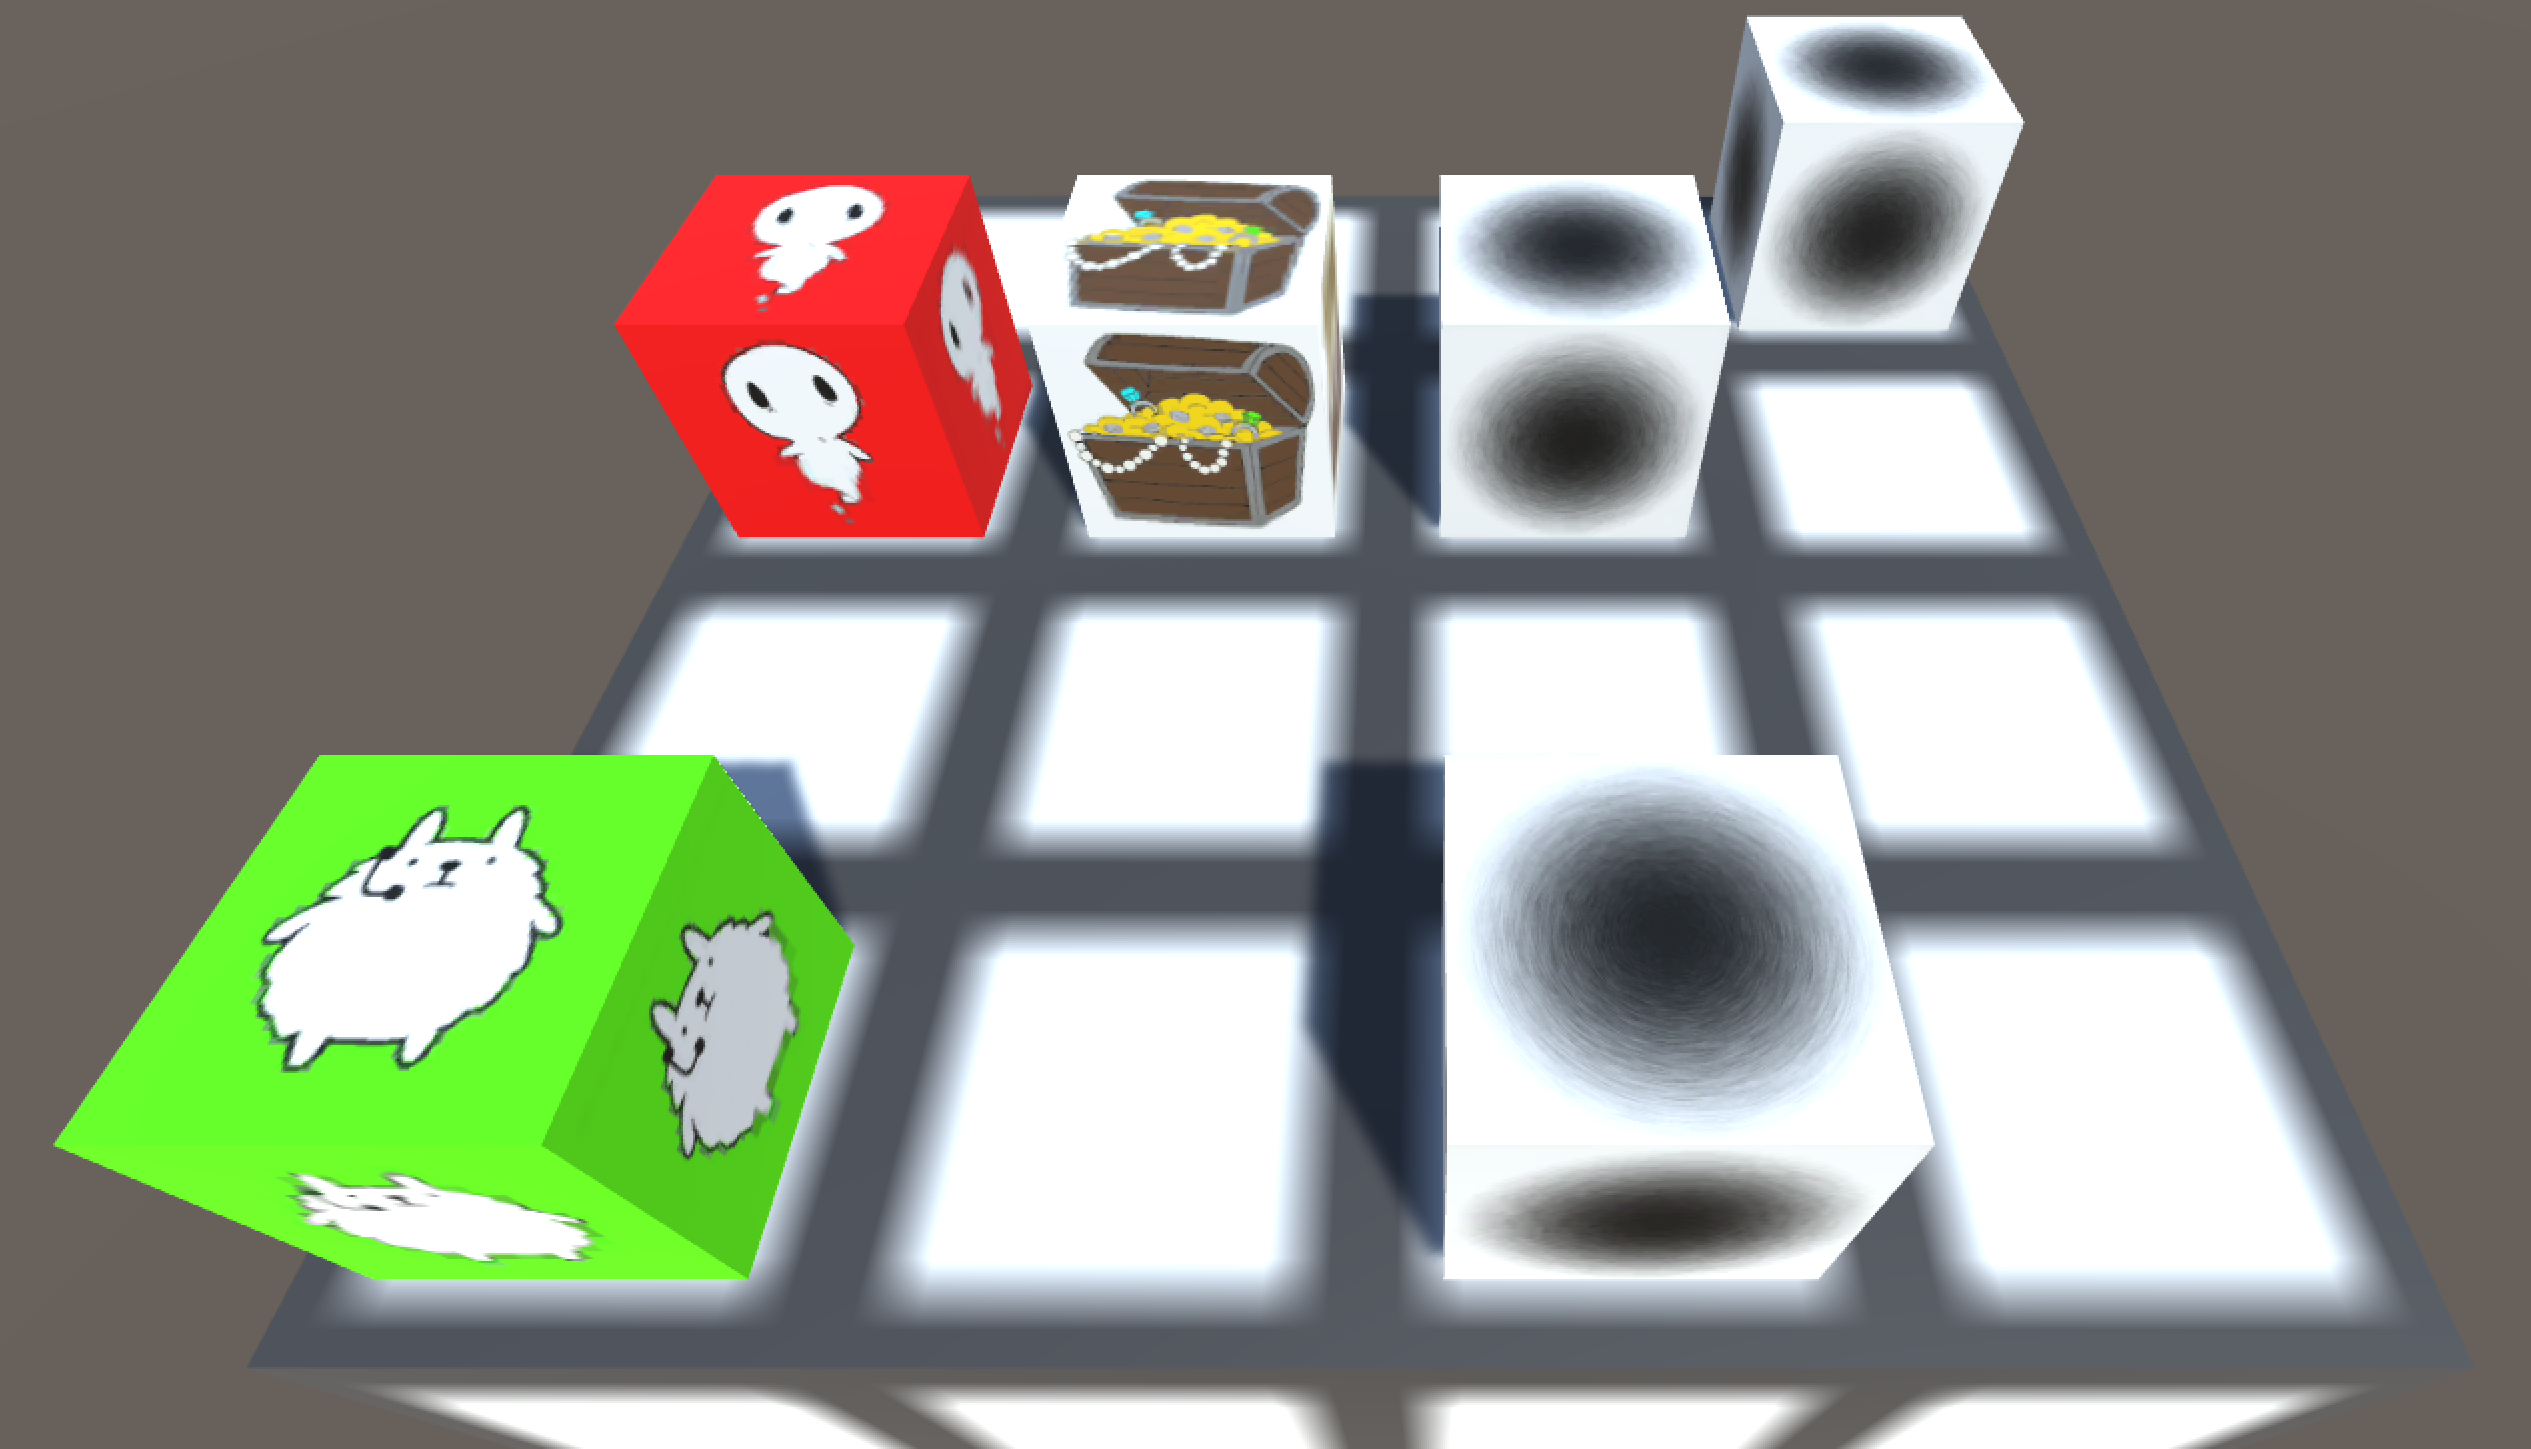
\includegraphics[width=\textwidth]{images/Wumpus_Unity.png}
    \caption{Wumpus implementation in Unity, the map is the same as in \figureref{wumpus:world}}
    \label{fig:wumpus:world:unity}
\end{figure}

\begin{figure}[H]
    \makebox[\textwidth][c]{
    \begin{tikzpicture}
    \tikzset{every mark/.append style={scale=.5}}
        \begin{axis}[
                width=1.25\textwidth, 
                height= 8cm,
                ylabel={Run time in microseconds},
                xlabel={Iteration No.},
                ymin = 0,
                ymax = 1500,
                xmin = 0,
                xmax = 130,
                ymajorgrids,
                legend columns = -1,
                area legend,
                legend style={draw=none,at={(0.5,1.05)},anchor=south, column sep=1ex}
            ]
            \addplot[mark=*, color=red] table [x={Iteration No.}, y=Unreal] {\macroData};
            \addplot[mark=*, color=blue] table [x={Iteration No.}, y=Unity] {\macroData};
            \legend{Unreal, Unity}
        \end{axis}
    \end{tikzpicture}}
    \caption{Wall clock-time for each invocation of the \ttt{World.Iterate}-method}
    \label{fig:macro-results}
\end{figure}
% Lua vs C++ in Lumberyard